% This is LLNCS.DEM the demonstration file of
% the LaTeX macro package from Springer-Verlag
% for Lecture Notes in Computer Science, version 1.1
\documentclass{llncs}
%\usepackage[numbers, sort&compress, square, comma]{natbib}
% \usepackage[lsnumbers, sort&compress, sEquare, comma]{natbib}    
% \usepackage{multirow}                             % not available on your system
\usepackage[table]{xcolor}
% \usepackage{amssymb}
\usepackage{amsmath}
\usepackage{graphicx}        % standard LaTeX graphics tool                            % when including figure files
\usepackage{multicol}        % used for the two-column index
\usepackage{multirow}
\usepackage{lscape}
\usepackage{float}
\usepackage{url}
\usepackage{caption,subfig}
\usepackage{graphicx}
\usepackage{amsmath}
\usepackage{amssymb}
\usepackage{color}
\usepackage{algorithm}
\usepackage{algorithmic}
\usepackage{tikz,graphicx}
\usepackage{url}
%\usepackage{etoolbox}
%\AtBeginEnvironment{algorithmic}{\small}
%

\graphicspath{{pictures/}} % Specifies the directory where pictures are stored

\def\dae{{\em Divide-and-Evolve}}
\def\DAE{{\sc DaE}}
\def\DAEX{{\sc DaE$_{\text{X}}$}}
%\def\DAEYAHSP{{\sc DaE$_{\text{YAHSP}}$}}
\newcommand{\DAEYAHSP}{{\sc DaE$_{\text{YAHSP}}$}}
\def\PARADISEO{{\sc ParadisEO-MOEO}}
\def\YAHSP{{\sc YAHSP}}
\def\modae{{\em Multi-Objective Divide-and-Evolve}}
\def\MODAE{{\sc MO-DaE}}
\def\ZENO{{\sc ZenoTravel}}
\def\MULTIZENO{{\sc MultiZenoTravel}}
\def\ZENOSOLVER{{\sc ZenoSolver}}
\def\PARAMILS{{\sc ParamILS}}

\begin{document}
%% Please leave SVN version number $Revision: 957 $
% Remember to enter the SVN command 
%      svn propset svn:keywords "Revision" thisFile.tex

\title{Pareto fronts for \MULTIZENO\ benchmarks -- $Revision: 957 $}

\author{A. Quemy \inst{1} \and M. Schoenauer\inst{1}\and
V. Vidal\inst{2}  \and J. Dr\'eo\inst{3} \and 
P. Sav\'eant\inst{2}}
% \author{Mostepha~R. Khouadjia \inst{1} \and Marc Schoenauer\inst{1}\and
% Vincent Vidal\inst{2}  \and Johann Dr\'eo\inst{3} \and Pierre Savéant\inst{3}}
%
\authorrunning{Alexandre Quemy et \textit{al.}} % abbreviated author list (for running head)
%
%%%% list of authors for the TOC (use if author list has to be modified)
\tocauthor{Alexandre Quemy, Marc Schoenauer, Vincent Vidal, Johann Dr\'eo, and Pierre Sav\'eant}
%
\institute{TAO Project, INRIA Saclay \&  LRI Paris-Sud University, Orsay, France\\%Universit\'{e} Paris-Sud
\email{\{alexandre.quemy, marc.schoenaue\}@inria.fr},\\ %WWW home page:
%\texttt{http://users/\homedir iekeland/web/welcome.html}
\and
ONERA-DCSD, Toulouse, France\\
\email{Vincent.Vidal@onera.fr}\\
 \and
 THALES Research \& Technology, Palaiseau, France\\
 \email{\{johann.dreo, pierre.saveant@thalesgroup.com\}}\\
}

\maketitle

\begin{abstract}
Contrary to single objective planning, multi-objective planning suffers from a lack of benchmarks with a known Pareto Front. As a result, testing and comparing algorithms is almost impossible. A method to generate various size tunable benchmarks for multi-objective planning with a known Pareto Front is proposed in order to provide a wide range of Pareto front shapes and different magnitudes of difficulty. The performances of the implementation are shown and some large instances with singular Pareto front shapes are proposed. A first attempt to solve some of them using multi-objective \DAEYAHSP\ solver is provided.
\end{abstract}
%
\section{Introduction}
\label{sec:intro}

Many benchmark suites exist for continuous multi-objective optimization (the famous ZDT, IHR, etc, proposed two decades ago), for which the exact Pareto front can be analytically computed, and with know difficulties (e.g. dimensionality, shape of the Pareto fronts, existence of local Pareto-optima, \ldots). For combinatorial optimization, the situation is not yet so clear, and whereas there exist known benchmark problems of all sizes, their Pareto fronts are generally not precisely known except the simplest ones (see e.g., MOCOLIB\footnote{\url{http://www.mcdmsociety.org/MCDMlib.html}}, offering several instances of several well-known combinatorial benchmark problems).

The context of the proposed benchmark suite is that of AI planning: a planning domain is defined by a set of predicates, that define the state of the system, a set of possible actions that can be triggered in states where their pre-conditions are satisfied, resulting in a new state. A planning problem instance is defined on a given planning domain by a list of objects, used to instantiate the predicates to define the state, an initial and a target state. The goal is to some up with a {\em feasible plan}, i.e., a set of actions that, when applied in turn to the initial state, lead the system to the goal state.

A simple planning problem in the domain of logistics, inspired by the well-known {\ZENO} problem of IPC series (see Figure \ref{fig.instance}) involves cities, passengers, and planes. Planes can fly from one city to another when a link exist, taking a given duration to do so (number on the link). Planes fly either empty, or carrying a unique passenger. An instance is defined by the number of cities and the links between them, a number of passengers and a number of planes. The goal of the (single-objective) planning problem is to carry all passengers from city I to city G in the minimum {\em makespan} (total duration of all flights). Because all planes can of course fly in parallel, this benchmark pertains to temporal planning. Previous work \cite{khouadjia:hal-00750560} proposed a multi-objective version of these benchmarks called \MULTIZENO, by adding a {\em cost} for landing in some cities: the second objective is to minimize the {\em total cost} of the plan. This work demonstrated the possibility for such 
problems to provide Pareto Front of various shapes and difficulties, but only provided the exact Pareto front for small instances.

This paper analyzes the \MULTIZENO\ benchamrks, providing an algorithm to compute the true Pareto Front even for very large instances. Beyond providing a generic way to generate Pareto Fronts of diverse complexity for AI Planning, the proposed \MULTIZENO\ benchmarks will allow testing different generic decomposition methods (weighted sum aggregation, Tchebycheff decomposition, Boundary Intersection approach) on large, concave, non-uniform, \ldots benchmarks of Combinatorial Multi-objective Problems of for which the Pareto Front is exactly known. 

The paper is organized as follows: Section \ref{sec:multizeno} formally presents the  \MULTIZENO\ benchmark, proving some properties of their Pareto optimal plans. Building on these properties, Section \ref{sec:zenosolver} proposes the \ZENOSOLVER\ algorithm to actually derive the true Pareto front for these instances. Sample experimental results demonstrate the diversity of Pareto fronts that can be obtained, and gives performance measurements of its complexity on large instances. The end of the paper presents experiments on some of the large \MULTIZENO\ instances obtained by Divide-and-Evolve, the only Pareto-based evolutionary AI planner to-date \cite{IJCAI2013}, which is rapidly recalled in Section \ref{sec:exp}, before some comparison with its single-objective version using the weighted sum aggregation on problems with non-convex fronts are given and discussed in Section \ref{sec:exp}.

\section{\MULTIZENO\ problem}
\label{sec:multizeno}
\subsection{Instances}

\begin{figure}
\centering
% \begin{tikzpicture}[thick,scale=1]
%     % Villes
%  \node[draw, fill=black!25] (0) at (-2,0) {$c_I$};
%  \node[draw, fill=black!25] (1) at (0,1.5) {$c_1$};
%  \node[draw, fill=black!25] (2) at (0,0) {$c_i$};
%  \node[draw, fill=black!25] (3) at (0,-1.5) {$c_n$};
%  \node[draw, fill=black!25] (4) at (2,0) {$c_G$};
% 
%     % Liaison inter villes
%  \draw[thick] (0) to[bend left] (1);
%  \draw[thick] (0)--(2) node[midway, above]{$d_i$};
%  \draw[thick, bend left] (0) to[bend right] (3);
%  
%  \draw[thick] (1) to[bend left] (4);
%  \draw[thick] (2)--(4) node[midway, above]{$d_i$};
%  \draw[thick] (3) to[bend right] (4);
%  
%  \draw[dashed] (1)--(2) node[midway, right]{$d_{1i}$};
%  \draw[dashed] (2)--(3) node[midway, right]{$d_{in}$};
%  \draw[thick] (1) to[bend right] (3);
%     
%     % Distance particulière
%  \node[] (A) at (-1.4,1.4) {$d_1$};
%  \node[] (A) at (1.4,1.4) {$d_1$};
%  \node[] (A) at (-1.4,-1.4) {$d_n$};
%  \node[] (A) at (1.4,-1.4) {$d_n$};
%  \node[] (A) at (-0.7,-0.7) {$d_{1n}$};
%  
% \end{tikzpicture}
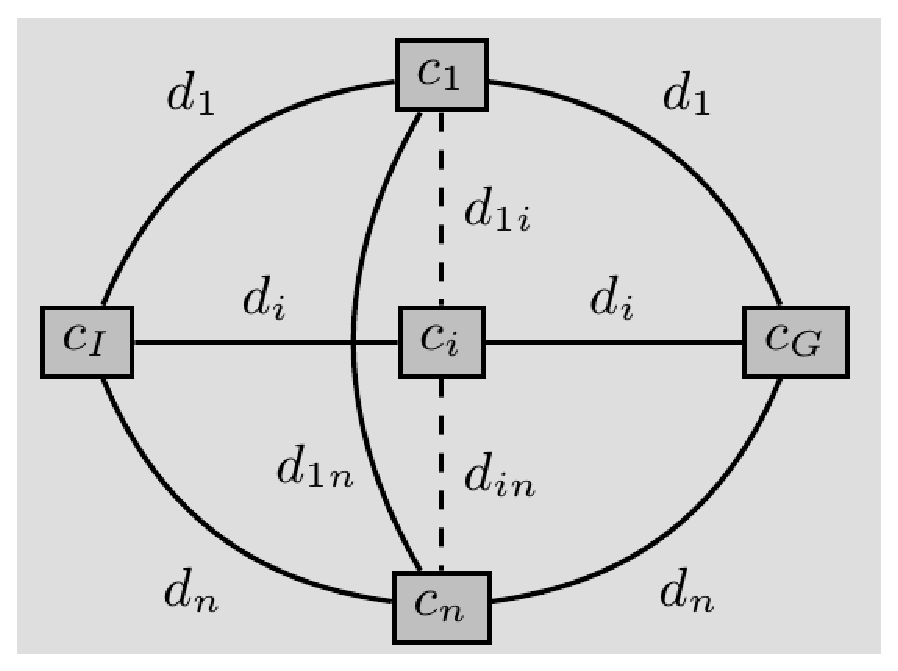
\includegraphics[width=0.5\textwidth]{abstractZeno.eps}
\caption{\label{fig.instance}A schematic view of a general \MULTIZENO\ problem. }
\end{figure}

Let us introduce some notations related to the planning problems introduced in Section \ref{sec:intro}: a \MULTIZENO\ instance (Figure \ref{fig.instance}) is defined by: $n$ 'central' cities, with costs $c_1, \ldots, c_n$\footnote{by abuse of notation, $c_i$ will denote both the city and the cost of landing in that city.}, plus the initial and goal cities $c_I$ and $c_G$; $t$ persons and $p$ planes, initially in $c_I$. Each central city provides a flight to the initial and final cities, with same flight durations $d_1, \ldots, d_n$. In addition, central cities form a clique, with durations $(d_{ij})_{i,j}, \forall (i,j) \in [1,n]^2$. The goal is to carry all persons to $c_G$, minimizing the makespan and the total cost of the plan.

%Without loss of generality, we can assume that the pairs $(d_i, c_i)$ are pairwise distinct (otherwise, the 2 cities can be ``merged'' and the resulting $n-1$ cities problem is equivalent to the original $n$ cities problem).

\subsection{Pareto Front}

\noindent
{\bf Proposition}: Possible Pareto-optimal plans are plans where using $2t-p$ cities.\\

{\bf Alternate tentative proof -- yet incomplete -- MS}\\
Some properties of the domain: \\
We have to assume that the {\em triangular inequality} is valid: for all triplet of cities $c_i, c_j, c_k$ (with $c_0=I$ and $c_{n+1}=G$), the makespans follow the triangular inequality $d_{ik} \leq d_{ij} + d_{jk}$ (with obvious notations for I and G).\\
A weaker form of this is the {\em shortest path} property, which is basically the triangular inequality with initial city I or G only (i.e. it's shorter to go from I or G directly to $c_i$ than to $c_j$ and then from $c_j$ to $c_i$.

We can then derive some properties that Pareto-optimal plans must fulfill:\\

Property 1 (obvious): No plane ever goes eastward (i.e., from G or to I) with a passenger.\\

Property 2: No plane ever goes westward empty.\\
Proof: Indeed, before going to I (resp. leaving G), it was in some central city $C_i$ and whatever the central city $C_j$ if goes to from I (resp. G), it could have gone there directly (same cost, lower makespan due to the triangular inequality.\\

Property 3: For any plane, no two subsequent flights involving a $C_i \rightarrow C_j$ flight can be both empty or both with a passenger.\\
Obvious due to the triangular inequality.

Corolary 1: Any passenger has to use a different planes for each segment of his trip (meaning that he has to wait some non-zero time at each central city he passes through).

In particular, if a passenger can only do a $I \rightarrow c_i \rightarrow c_j \rightarrow G$ trip by using 3 different planes -- and this case is true even with only the {\em shortest path} property.\\
{\em y'a plus que ce cas-l\`a \`a traiter pour montrer qu'un passager ne passe que par une seule ville centrale}
 
Property 4: the last passenger to reach G is picked up in some $C_i$ by a plane coming from G or by the same plane that brought him from I.\\
{\em je ne sais pas si \c{c}a sert \`a quelque chose pour la suite, pas trouv\'e de r\'ecurrence}.\\


{\bf Alternate Alexandre's proof}:
We consider a passenger using 2 central cities (but the reasoning can be extended to any number of cities), $c_i$ and $c_j$. The path he follows must involve 1, 2 or 3 planes. With a single plane, we can obviously reduce $c_I \to c_i \to c_j \to c_G$ with a duration $d_i+d_{ij}+d_j$ to $c_I \to c_i \to c_G$ with a smaller cost and duration.
With two planes, one of them will perform the following pattern $c_I \to c_i \to c_j$ or $c_i \to c_j \to c_G$. Then, we can reduce it to $c_I \to c_j$ or $c_i \to c_G$ with a smaller cost and a better duration.

With 3 planes, we obtain the following schedule:

\begin{center}
\begin{tabular}{c l}
    $p_1:$ & $\ldots \to c_I \to c_i \to \ldots$\\
    $p_2:$ & $\ldots \to c_i \to c_j \to \ldots$\\
    $p_3:$ & $\ldots \to c_j \to c_G \to \ldots$\\
\end{tabular}
\end{center}

However, as $d_{ij} > d_i + d_j$ we can modify the schedule of the second plane with $p_2: \ldots \to \ldots c_i \to c_G \to c_j \to \ldots$.

The cost of the plan is not modified, but the makespan can be lower (or in the worst case the same). Finally, the passenger used only one central city.

We prove now that we can suppress every flight between two central cities. A flight between 2 central cities is performed by an empty plane. Otherwise, a passenger would have flown through more than one city.

As a passenger will use only one city, it involves 1 or 2 planes. With the same argument as previously, the case with a single plane is trivial. With two planes, if a plane uses an edge between two central cities $c_i$ and $c_j$, it means that it brings a passenger to $c_i$ (otherwise it could have flight directly to $c_j$), and thus is coming from $c_I$. 

\begin{center}
\begin{tabular}{c l}
    $p_1:$ & $\ldots \to c_I \to c_i \to c_j \to c_G \to \ldots$\\
    $p_2:$ & $\ldots \to c_I \to c_j \to \ldots$\\
\end{tabular}
\end{center}

As $d_{ij} > d_i + d_j$, we can replace the edge $c_i \to c_j$ by the path $c_i \to c_I \to c_j$ which is better regarding durations.

In conclusion, each person uses only one central city and we can always suppress flights between two central cities. Hence, Possible Pareto-optimal plans uses $2t-p$ cities.

{\bf Original Alexandre's proof}: Let us consider a feasible plan $P$ using $2t-p+k$ cities. At least one passenger will land in more than one city and thus, a plane will fly between two central cities. A flight between two central cities can be performed by an empty plane or a plane with a passenger. In the first case, the plane will perform a pattern $c_{i_1} \to c_{i_2} \to c_{i_3}$ with $c_{i_2}$ a central city, as well as $c_{i_1}$ or $c_{i_3}$. We can reduce that path to $c_{i_1} \to c_{i_3}$ and then reducing the cost of the total plan by $c_{i_2}$. Obviously, the plan is still feasible. Regarding the makespan, if the plane was not the one with the higher duration, the makespan does not change. If it was, in the worst case, the plane will have to wait the duration $d_{i_2}$. Hence, in the worst case, the makespan remains the same but cannot be higher.

For the second case, we consider the path followed by a passenger from $c_1$ to $c_G$, in the plan $P$. Such a path is caracterised by a vector in $\mathbb{N}^{K}$ where $K$ is the number of cities the passenger will visit. A passenger will be carried out by $m \in \mathbb{N}^*$ planes: $K = \sum_{i=1}^m k_i$ and the path can be expressed as follows: 
$$\underbrace{c_I \to c_{i_{1}} \to \ldots \to c_{i_{k_1}}}_{\text{First plane}} \underbrace{\to c_{i_{k_1 + 1}} \to \ldots}_{\text{Second plane}} \to c_{i_{k_2}} \to \ldots \to c_{i_{k_m}} \to c_G$$
We can reduce each part of the path $c_{i_{k_j}} \to \ldots \to c_{i_{k_{j-1}}}$ to the path $c_{i_{k_j}} \to c_{i_{k_{j-1}}}$. With the same argument, the plan is still valid and, in the worst case, the cost of the entire plan remains the same (if the considered passenger follows a path with only one central city), as well as the makespan. However none of the two objectives can be worse than the previous plan.

By this procedure, we are removing all edges between two central cities. As a result, we will have a feasible plan, with the minimum number of cities needed to carry out $t$ passengers, that is to say $2t-p$. In the worst case, the cost is lower and the makespan are the same as the intial plan $P$. $\square$\\

\noindent
{\bf Corollary}: possible Pareto-optimal plans and plans where each person visits only one central city.

\subsection{Pareto-optimal Plans}
A Possibly Pareto-optimal Plan (PPP) is thus defined by 2 tuples, namely $e \in [0,n]^t$ for cities involved in eastbound flights, and $w \in [0,n]^{t-p}$ for westbound flights, and a schedule for the corresponding $4t-2p$ arcs. Note that there exists many feasible schedules, i.e., schedules that actually are feasible plans for $p$ planes. There are at most $n^{(2t-p)}$ possible PPP. However, such set contains many redundancies, that can easily be removed by ordering the indices:\\

\noindent
{\bf Definition}: considering $E = \{e \in [0,n]^t ~|~ \forall i \in [1,t-1], d_{e_i} \geq d_{e_{i+1}}\}$ and $W = \{w \in [0,n]^{t-p} ~|~ \forall i \in [1,t-1],  d_{w_i} \geq d_{w_{i+1}}\}$ an {\it admissible} PPP is an element of $E \times W$.\\

\noindent
{\bf Number of admissible PPP}: Let consider the space $\Gamma^{m}_{k}$ of $m$-tuples such that $\forall u \in \Gamma^{m}_{k} \;\; ||u||_1 = k$. The cardinality of $\Gamma^{m}_{k}$ is the number of combinaisons with repetitions of $k$ elements into a set of $m$, i.e. ${m+k-1 \choose k}$. As it exists a bijection between $E$ and $\Gamma^{n}_{t}$ and another between $\Gamma^{n}_{t-p}$ and $W$, we can conclude that the number of PPP is the cardinality of $\Gamma^{n}_{t} \times \Gamma^{n}_{t-p}$, i.e. ${n+t-1 \choose t}{n+(t-p)-1 \choose t-p}$.\\

\noindent
{\bf Cost of a PPP}: Given a PPP C, the cost of {\bf any} plan using (only) these cities are uniquely determined by $ \text{Cost}(C) = \underset{{e_i \in e}}{\sum} c_{e_i} + \underset{{w_i \in w}}{\sum} c_{w_i}$.\\

\noindent
{\bf Makespan of a PPP}: The makespan of the PPP is thus that of the shortest schedule that uses the $4t-4$ arcs in a feasible way. Trivial upper and lower bounds for the shortest makespan of a PPP $C$ are respectively $M_S(C)$, the makespan of the sequential plan (i.e., that of the plan for a single plane that would carry all persons one by one), and $M_L(C)$, the makespan of the perfect plan where none of the $p$ planes would ever stay idle. These bounds are useful to prune PPP.

$$M_S(C) = 2 (\underset{{e_i \in e}}{\sum} d_{e_i} + \underset{{w_i \in w}}{\sum} d_{w_i}) ~~~~~~~~~~~~~~~~ M_L(C) = \frac{M_S(C)}{p}$$

\noindent
{\bf Greedy domination}: Given two PPP $C$ and $C'$, $C$ {\it greedily dominates} $C'$ if $M_S(C) \leq M_L(C')$ and $Cost(C) \leq Cost(C')$.

\subsection{Computing the Shortest Makespan}
%\subsubsection{Flight patterns}

\begin{figure}
\centering
% \begin{tikzpicture}[thick,scale=0.4]
%     % Villes
%  \node[draw, fill=black!25] (0) at (-3.5,0) {\large $c_0$};
%  \node[draw, fill=black!25] (2) at (0,0) {\large $c_i$};
%  \node[draw, fill=black!25] (4) at (3.5,0) {\large $c_G$};
% 
%     % Liaison inter villes
%  \draw[thick] (0)--(2) node[midway, above]{$d_{i}$};
%  \draw[thick] (2)--(4) node[midway, above ]{$d_{i}$};
% 
%  \draw[thick,->,>=stealth, red] (0.20) -- (2.160);
%  \draw[thick,->,>=stealth, red] (2.20) -- (4.160);
% \end{tikzpicture}
% %\caption{\label{M1} Pattern 1}
% \begin{tikzpicture}[thick,scale=0.4]
%     % Villes
%  \node[draw, fill=black!25] (0) at (-3.5,0) {\large $c_0$};
%  \node[draw, fill=black!25] (2) at (0,0) {\large $c_i$};
%  \node[draw, fill=black!25] (4) at (3.5,0) {\large $c_G$};
% 
%     % Liaison inter villes
%  \draw[thick] (0)--(2) node[midway, above]{$d_{i}$};
%  \draw[thick] (2)--(4) node[midway, above]{$d_{i}$};
% 
%  \draw[thick,<-,>=stealth, red] (0.20) -- (2.160);
%  \draw[thick,<-,>=stealth, red] (2.20) -- (4.160);
% \end{tikzpicture}
% %\caption{\label{M2} Pattern 2}
% \begin{tikzpicture}[thick,scale=0.4]
%     % Villes
%  \node[draw, fill=black!25] (0) at (-3.5,0) {\large $c_0$};
%  \node[draw, fill=black!25] (2) at (0,0) {\large $c_i$};
%  \node[draw, fill=black!25] (4) at (3.5,0) {\large $c_G$};
% 
%     % Liaison inter villes
%  \draw[thick] (0)--(2) node[midway, above]{$d_{i}$};
%  \draw[thick] (2)--(4) node[midway, above]{$d_{i}$};
% 
%  \draw[thick,->,>=stealth, red] (0.20) to[left] (2.160);
%  \draw[thick,<-,>=stealth, red] (0.-20) to[right] (2.200);
% 
%   \draw[thick,->,>=stealth, blue] (2.380) to[left] (4.160);
%  \draw[thick,<-,>=stealth, blue] (2.340) to[right] (4.200);
% \end{tikzpicture}
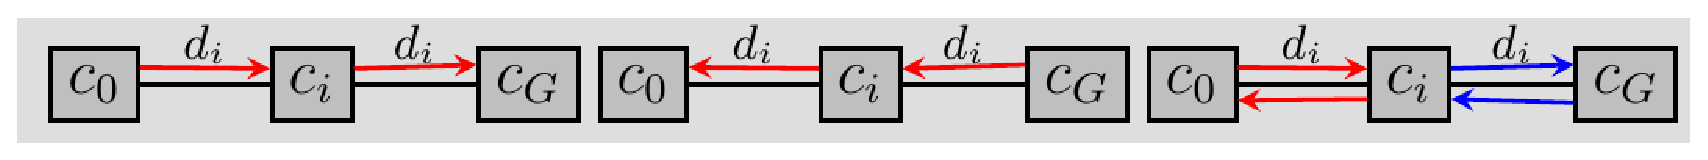
\includegraphics[width=0.8\textwidth]{patternsZeno.eps}
\caption{\label{M3} Respectively Pattern 1,2 and 3.}
\end{figure}
%,->,>=stealth

It exists 3 different patterns that can be carried out by planes, represented by Fig. \ref{M3}. We can notice that the last one has to be performed by two planes and is non-preemptive (i.e. once the first plane drops off the person at the central city, the other plane can pick her up later).

We will denote the cardinal of the first and the second pattern in a PPP by, respectively, $\alpha_E$ and $\alpha_W$ and for last pattern by $\beta$. We will refer to the eastern part and the western part of $\beta$ by, respectively, $\beta_E$ and $\beta_W$. Notice that it is possible for a given $\beta$ to have multiple choices for the cities involved in Pattern 3. Each choice is denoted $\beta_{set}$ and the set of $\beta_{set}$ the $\beta$-PowerSet. However, given $\beta$, the number of each pattern is fully qualified: 
$$
\left\{
\begin{matrix}
\alpha_W = t-p-\beta \\
\alpha_E = t - \beta \\
\end{matrix}\right.$$



%\subsubsection{The method}
The optimal makespan for a given admissible PPP $C$, is the lowest makespan obtained for all $\beta_{set} \in \beta$-PowerSet. For each $\beta_{set}$ we solve a subproblem without Pattern 3. Then we take into account Pattern 3. We prove the obtained makespan is optimal even if we solve two differents problems with greedy algorithms.
%\subsubsection{Subproblem} 

For a given $\beta_{set}$ and PPP $C$, we denotes by $e' = e - \beta_{set}$ where the result is the tuple $e$ such that we deleted elements of $\beta_{set}$ and $w' = w - \beta_{set}$. Thus, we have a new PPP $C'$ with $\beta' = 0$, i.e without Pattern 3. 
The greedy Algorithm \ref{subproblem} returns the optimal makespan for a PPP and $\beta = 0$.

\begin{algorithm}
\caption{\label{subproblem} Optimal makespan for $\beta = 0$}
\begin{algorithmic}
%\REQUIRE $n \geq 0 \vee x \neq 0$
%\ENSURE $y = x^n$
\STATE $maxE \leftarrow 0$
\STATE $maxW \leftarrow t$
\STATE $D_i \leftarrow 0 \; \forall i=1,\ldots,p$
\STATE $S_i \leftarrow EAST \; \forall i=1,\ldots,p$
\COMMENT {Indicates the direction for the next flight of the plane i.}

\WHILE{$maxW \neq 2t-p$}
\STATE $k \leftarrow \underset{i}{argmin}(D_i)$ \COMMENT {First plane waiting (ie. arriving at $c_I$ or $c_G$)}
\IF{$S_k = EAST$}
\STATE $D_k \leftarrow D_k + 2d_{c_{maxE}}$
\STATE $S_k \leftarrow WEST$
\STATE $maxE \leftarrow maxE + 1 $;
\ELSE
\STATE $D_k \leftarrow D_k + 2d_{c_{maxW}}$
\STATE $S_k \leftarrow EAST$
\STATE $maxW \leftarrow maxW + 1 $;
\ENDIF
\ENDWHILE
\\
\WHILE{$maxE \neq t$}
\STATE $k \leftarrow \underset{i, S_i=EAST}{argmin}(D_i)$
\STATE $D_k \leftarrow M_k + 2d_{c_{maxE}}$
\STATE $S_k \leftarrow WEST$
\STATE $maxE \leftarrow maxE + 1 $;
\ENDWHILE
\\
\RETURN $\underset{i}{max}(D_i)$
\end{algorithmic}
\end{algorithm}

%\subsubsection{Tackling Pattern 3}
The second step of the algorithm is to dispatch durations of Pattern 3 between planes according to $(D_i)_i$ computed for the associated subproblem. This can be performed greedily by chosing the longest flight and adding this duration the two planes with the smallest current duration.\\

{\bf Example}: $t=7$, $p=3$, $d=(2,4,6), C = (3,3,2,2,2,1,1)(3,3,2,1) \implies 0 \leq \beta \leq 3$.\\
If we chose $\beta_{set} = \{3,2,1\}$, then, $C' = (3,2,2,1)(3)$, with only $t=4$.\\

\begin{tabular}{c l c}
Step 1 without Pattern 3 & $~~~~~~~~~~~~~~~~~~~~~~~~~~$ & Step 2 including Patterns 3
\tabularnewline
\begin{tabular}{|c | l | c|}
    \hline
    $p_1$ & $D_{1} = 12$ \tabularnewline
    $p_2$ & $D_{2} = 24$ \tabularnewline
    $p_3$ & $D_{3} = 8$ \tabularnewline
    \hline
\end{tabular} 
&  &
\begin{tabular}{|c | l |}
    \hline
    $p_1$ & $D_{1} =32$ \tabularnewline
    $p_2$ & $D_{2} = 28$ \tabularnewline
    $p_3$ & $D_{3} = 32$ \tabularnewline
    \hline
\end{tabular}
\end{tabular}\\\\

\noindent
Hence, the optimal makespan is 32.\\

If the plane that picks the passenger up from the central city arrived before the passenger has been carried out by the first plane, this plane has to wait and then, it is possible that the makespan of the plan is not simply a greedy distribution of durations.\\

\noindent
{\bf Proposition}: We can always construct a valid plan with the makespan returned by the described method.\\

{\bf Proof by construction}: The idea is to satisfy as soon as possible time requirement for each Pattern 3 by performing western parts as soon as possible, and to perform eastern parts as late as possible.
Considering a pattern 3 performed by plane $p_1$ et $p_2$, through city $c_i$ their schedules look like:

\begin{center}
\begin{tabular}{c l l}
    $p_1:$ & $c_I \to \ldots \to c_G \to \overset{\blacklozenge}{c_i} \to c_G \to \ldots \to c_G$\tabularnewline
    $p_2:$ & $c_I \to \ldots \to c_I \to \overset{\lozenge}{c_i} \to c_I \to \ldots \to c_G$\tabularnewline
\end{tabular}
\end{center}
~\\\noindent
We denote by $\blacklozenge$ a possible waiting point and by $\lozenge$ the moment where the passenger arrived in city $c_i$. The time requirement (t.r.) is the time needed for $p_2$ to bring the passenger to $c_i$, i.e. the duration before $\lozenge$.

Let us consider only planes such that they have to perform at least a Pattern 3 (otherwise the construction is trivial).

\begin{enumerate}
\item For each plane, select the one with the maximum number of Pattern 3 to be performed. In case of equality, select the plane such the Pattern 3 duration is the highest, or the plane with the longer duration.
\item Construct a partial schedule with only Pattern 1 and 2. 
\item For each not already started Pattern 3, add the eastern part at the end of the schedule by descending order durations.
\item For each already started Pattern 3, add the western part at the begining of the schedule by ascending order durations. $\square$
\end{enumerate}

{\bf Example}:

\begin{center}
\begin{tabular}{l c r}

\begin{tabular}{|c | c | c|}
    \hline
    $p_i$ & $D_i$ & Pat. 3 \tabularnewline
    \hline
    $p_1$ & $32$ & 2 \tabularnewline
    $p_2$ & $28$ & 1 \tabularnewline
    $p_3$ & $32$ & 3 \tabularnewline
    \hline
\end{tabular} & ~~ &
\begin{tabular}{c l l}
    $p_3:$ & $c_I \to c_2 \to c_G \to \overset{\blacklozenge_3}{c_3} \to c_G \to \overset{\blacklozenge_2}{c_2} \to c_G \to \overset{\blacklozenge_1}{c_1} \to c_G$\tabularnewline
    $p_2:$ & $c_I \to c_1 \to c_I \to c_2 \to c_G \to c_3 \to c_I \to c_2 \to c_G$\tabularnewline
    $p_3:$ & $c_I \to c_3 \to c_I \to c_2 \to c_I \to c_3 \to c_G$\tabularnewline
\end{tabular}

\end{tabular}
\end{center}



\noindent
{\bf Proposition}: The makespan returned by the algorithm is optimal for the PPP C and the cities involved in the pattern 3.\\

{\bf Proof}: The incompressible time to transport all passengers, according to a given $\beta_{set}$ is $T = 4\underset{i\in \beta_{set}}{\sum} d_i + 2\underset{i\in \{ e',w' \}}{\sum} d_i$. A theoretical optimal plan with this pattern repartition is a plan without any waiting point for any plane.
The above algorithm gives the optimal distribution of the set of times into $p$. Then, if a plan can be constructed with such a makespan, it is optimal for the PPP and the repartition of patterns.
As it exists a method to construct such a plan, we can conclude that the algorithm is optimal for the PPP C and $\beta_{set}$. %We can also conclude that, in this case, it is always possible to construct a plan without any waiting point. 
$\square$\\

\noindent
{\bf Number of iterations by PPP}: In the worst case, for each value of $\beta$ we have then ${t-p \choose \beta}$ possibilities. Then, we will perform $2^{t-p}$ iterations. 

\section{\ZENOSOLVER}
\label{sec:zenosolver}
\ZENOSOLVER\ is a C\texttt{++11} software dedicated to solve \MULTIZENO\ instances. It allows to tune every parameters in order to adjust the difficulty or to obtain different shapes for Pareto Front. Furthermore, it can generate \texttt{PDDL} files for easy-to-use instances.
\ZENOSOLVER\ proposes an implemention of the method described in this paper, namely Algorithm \ref{alg:zeno}, that consists to iterate over $E \times W$ without any explicit construction of the admissible-PPP set.

The vectors $c$ and $d$ are generated thanks to two functions, $f$ and $g$, provided by the user, such that $c_i = x_cf(a_ci+b_c)+y_c$ and $d_i = x_dg(a_di+b_d)+y_d$. However, $d$ is generated by a backward iterator to insure that objectives are contradictory. Scale and translation constants allow a deeper control of the front shape and are set, respectivly, to 1 and 0 by default.

\begin{algorithm}
\caption{\label{alg:zeno}\ZENOSOLVER: main algorithm.}
\begin{algorithmic}
%\REQUIRE $n \geq 0 \vee x \neq 0$
%\ENSURE $y = x^n$
\STATE Initialise $S$ a map indexed by costs.
\FORALL{$e\in E$}
    \FORALL{$w\in W$}
        \IF{PPP made from $e$ and $p$ is not dominated regarding $S$}
            \STATE Calculate optimal makespan for this PPP.
            \STATE Insert the makespan if it is better than the previous for the same cost.
        \ENDIF
    \ENDFOR
\ENDFOR
\STATE Extract the exact Pareto front from $S$.
\end{algorithmic}
\end{algorithm}
Determining if the current PPP is dominated can be performed in $O(h)$ where $h$ is the size of $S$. 
%The insertion is in $O(log~h)$ but could be reduced to $O(1)$ using a "hint" for insertion. 
The insertion is in $O(log~h)$. 
An obvious upper-bound on the size of $S$ is given by $(2t-p)(\underset{i}{max}(c_i) - \underset{i}{min}(c_i))$.

\subsection{Performances}

The number of iterations is influenced by the number of PPP but also by the structure of PPP. If we increase $n$, we do not increase the number of iterations for a lot of PPP. Moreover, the upper-bound by PPP is $2^{t-p}$, hence, it is not influenced by $n$. On the contrary, if we increase $t$, the upper-bound grows up and the average number of iterations per PPP will also increase.

The Figure \ref{speed1} shows that difference on the time using a i3 CPU M 380 @ 2.53GHz. The Figure \ref{ratio1} confirms the pruning method effect. In addition, it really shows that the number of iterations follows the number of PPP if we increase $n$, but explodes if we increase $t$. We can notice that increasing $n$ while using the pruning method results in a worse time, even if the ratio is better (we are performing less iterations than PPP). This is due to the fact that the cost of the pruning method is higher than its benefit. In addition, even if instances are faster to be solved with the pruning method in the case of $t$, it appears the gain is not significant. This behavior is instance dependant. Indeed, Figure \ref{speed1} and \ref{ratio1} are based on instances such that $f(i) = g(i) = i$ resulting in a linear front. Same experiment, with $f(i) = g(i) = log(i)$ results in Figure \ref{speed2} leading to a more optimistic conclusion.

\begin{figure}[h!]
  \centering
      \includegraphics[width=0.30\textwidth]{speed_T}
      \includegraphics[width=0.30\textwidth]{speed_N}
 \caption{\label{speed1} Time function of $t$ (left) or $n$ (right).}
\end{figure}
\begin{figure}[h!]
  \centering
      \includegraphics[width=0.30\textwidth]{ratioIte_T}
      \includegraphics[width=0.30\textwidth]{ratioIte_N}
    \caption{\label{ratio1} Ratio of iterations over number of PPP, function of $t$ (left) or $n$ (right).}
\end{figure}
\begin{figure}[h!]
  \centering
      \includegraphics[width=0.30\textwidth]{speed_log_T}
      \includegraphics[width=0.30\textwidth]{ratioIte_log_T}
    \caption{\label{speed2} Time and ratio for a different instance (concave front).}
\end{figure}

Early experimentation using an explicit instanciation of the set $E \times W$ resulted in a lack of memory, even for medium instances. As we are never creating other PPP that the one we are working on with Algorithm \ref{alg:zeno}, the memory usage is now limited by the size of $S$, i.e. approximativly the size of the Pareto Front (see Table \ref{table:i}). 

\begin {table}[H]
\centering
\caption{\label{table:i} Increasing simultaneously $n$ and $t$ with $f(i)=g(i)=i$.}
\begin{tabular}{|c|c|c|c|c|c|c|c|}
  \hline
  n & t & p & PPP Size & Iterations & $S$ Size & Front Size & Time (ms)\\
  \hline
  3 & 3 & 2 & 30 & 33 & 9 & 5 & 0\\
  4 & 4 & 2 & 350 & 408 & 19 & 10 & 1\\
  5 & 5 & 2 & 4410 & 6387 & 33 & 17 & 6\\
  6 & 6 & 2 & 58212 & 109831 & 51 & 26 & 117\\
  7 & 7 & 2 & 792792 & 1930385 & 73 & 37 & 2278\\
  8 & 8 & 2 & 11042460 & 34648348 & 99 & 50 & 43572\\
  9 & 9 & 2 & 156434850 & 630225670 & 129 & 65 & 1036772 \\
  10 & 10 & 2 & 2245709180 & 11600589455 & 163 & 82 & 20785211 \\
  \hline
\end{tabular}
\end{table}

\begin {table}[H]
\centering
\caption{\label{table:loglog} Increasing simultaneously $n$ and $t$ with $f(i)=g(i)=log(i)$.}
\begin{tabular}{|c|c|c|c|c|c|c|c|c|c|}
  \hline
  n & t & p & PPP Size & \multicolumn{2}{c|}{Iterations} & $S$ Size & Front Size & \multicolumn{2}{c|}{Time (ms)} \\
  \hline
    3 & 3 & 2 & 30 & 48 & 36 & 15 & 5 & 0 & 0\\
    4 & 4 & 2 & 350 & 770 & 314 & 74 & 10 & 0 & 0\\
    5 & 5 & 2 & 4410 & 12810 & 1323 & 389 & 19 & 12 & 3\\
    6 & 6 & 2 & 58212 & 219912 & 3050 & 890 & 29 & 207 & 25\\
    7 & 7 & 2 & 792792 & 3868032 & 6376 & 1322 & 36 & 6613 & 276\\
    8 & 8 & 2 & 11042460 & 69320988 & 12226 & 1785 & 54 & 127332 & 3918\\
    9 & 9 & 2 & 156434850 & 1260758070 & 26128 & 2276 & 77 & 2283654 & 58104\\
    10 & 10 & 2 & 2245709180 & 23202174710 & 50428 & 2781 & 111 & 46723743 & 955131\\
  \hline
\end{tabular}
\end{table}

\begin {table}[H]
\centering
\caption{\label{table:logsqrt} Increasing simultaneously $n$ and $t$ with $f(i)=log(i)$ and $g(i)=\sqrt i$.}
\begin{tabular}{|c|c|c|c|c|c|c|c|c|c|}
  \hline
  n & t & p & PPP Size & \multicolumn{2}{c|}{Iterations} & $S$ Size & Front Size & \multicolumn{2}{c|}{Time (ms)} \\
  \hline
    3 & 3 & 2 & 30 & 48 & 36 & 15 & 5 & 0 & 0\\
    4 & 4 & 2 & 350 &  770 & 368 & 83 & 10 & 0 & 0\\
    5 & 5 & 2 & 4410 & 12810 & 2297 & 409 & 19 & 11 & 9\\
    6 & 6 & 2 & 58212 & 219912 & 4881 & 857 & 36 & 207 & 24\\
    7 & 7 & 2 & 792792 & 3868032 & 8956 & 1349 & 37 & 6237 & 266\\
    8 & 8 & 2 & 11042460 & 69320988 & 19888 & 1856 & 65 & 120383 & 3526\\
    9 & 9 & 2 & 156434850 & 1260758070 & 36756 & 2482 & 83 & 2240856 & 52954\\
    10 & 10 & 2 & 2245709180 & 23202174710 & 65359 & 3144 & 104 & 46216951 & 1161831\\
  \hline
\end{tabular}
\end{table}

\begin {table}[H]
\centering
\caption{\label{table:sqrtlog} Increasing simultaneously $n$ and $t$ with $f(i)=\sqrt i$ and $g(i)=i$.}
\begin{tabular}{|c|c|c|c|c|c|c|c|c|c|}
  \hline
  n & t & p & PPP Size & \multicolumn{2}{c|}{Iterations} & $S$ Size & Front Size & \multicolumn{2}{c|}{Time (ms)} \\
  \hline
    3 & 3 & 2 & 30 & 48 & 36 & 9 & 5 & 0 & 0\\
    4 & 4 & 2 & 350 & 770 & 419 & 19 & 10 & 0 & 0\\
    5 & 5 & 2 & 4410 & 12810 & 3014 & 33 & 17 & 10 & 3\\
    6 & 6 & 2 & 58212 & 219912 & 14739 & 51 & 26 & 223 & 25\\
    7 & 7 & 2 & 792792 & 3868032 & 48512 & 73 & 37 & 6510 & 163\\
    8 & 8 & 2 & 11042460 & 69320988 & 47838 & 99 & 65 & 115977 & 1709\\
    9 & 9 & 2 & 156434850 & 1260758070 & 119686 & 129 & 65 & 2222907  & 26661\\
    10 & 10 & 2 & 2245709180 & - & 195214 & 163 & 110 & - & 702926\\
  \hline
\end{tabular}
\end{table}

\begin {table}[H]
\centering
\caption{\label{table:f5} Increasing simultaneously $n$ and $t$ with $f(i)=g(i)=\frac{5}{2}i + \frac{(i ~\text{mod}~ 2)}{10}$.}
\begin{tabular}{|c|c|c|c|c|c|c|c|c|c|}
  \hline
  n & t & p & PPP Size & \multicolumn{2}{c|}{Iterations} & $S$ Size & Front Size & \multicolumn{2}{c|}{Time (ms)} \\
  \hline
    3 & 3 & 2 & 30 & 48 & 30 & 15 & 6 & 0 & 0\\
    4 & 4 & 2 & 350 & 770 & 622 & 84 & 20 & 0 & 0\\
    5 & 5 & 2 & 4410 & 12810 & 2245 & 369 & 31 & 12 & 3\\
    6 & 6 & 2 & 58212 & 219912 & 172759 & 890 & 115 & 222 & 349\\
    7 & 7 & 2 & 792792 & 3868032 & 166183 & 1875 & 121 & 6639 & 785\\
    8 & 8 & 2 & 11042460 & 69320988 & 51806458 & 3335 & 366 & 114788 & 235221\\
    9 & 9 & 2 & 156434850 & 1260758070 & 10530973 & 5435 & 233 & 2154571 & 176702\\
  \hline
\end{tabular}
\end{table}

\subsection{Instances}
We propose six large instances with totaly different front shapes and complexities (on the left side, a zoom on a part of the front) to demonstrate the possibilities of \ZENOSOLVER. The generating time strongly varies from some minutes (2 minutes for Instance 1) up to hours (17h for Instance 3). 

\begin{figure}[h!]
  \centering
      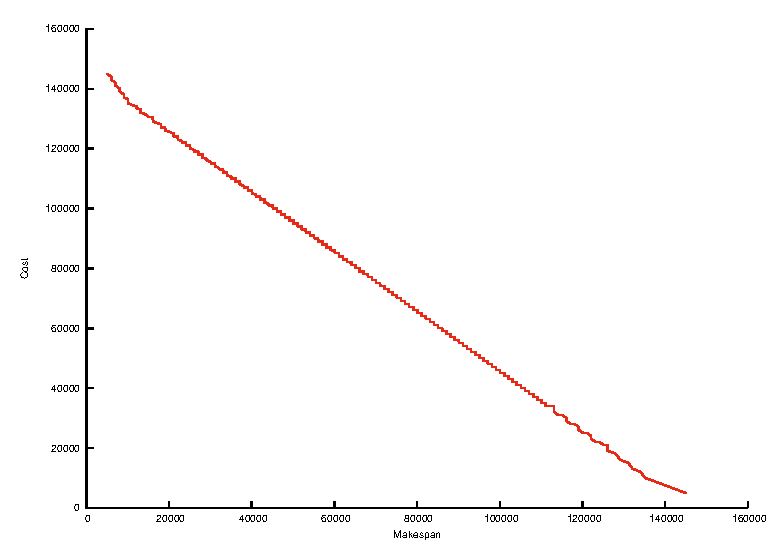
\includegraphics[width=0.30\textwidth]{1}
      \includegraphics[width=0.30\textwidth]{1_zoom}
 \caption{\label{instance1} Instance 1: the trend appears to be linear with some convex parts on extremities. However, a zoom shows a totaly unstructured front.}
\end{figure}
\begin{figure}[h!]
  \centering
      \includegraphics[width=0.30\textwidth]{4}
      \includegraphics[width=0.30\textwidth]{4_zoom}
 \caption{\label{instance2} Instance 2: a convex trend. The lower part is totally linear while the upper part is made of regular concave patterns.}
\end{figure}
\begin{figure}[h!]
  \centering
      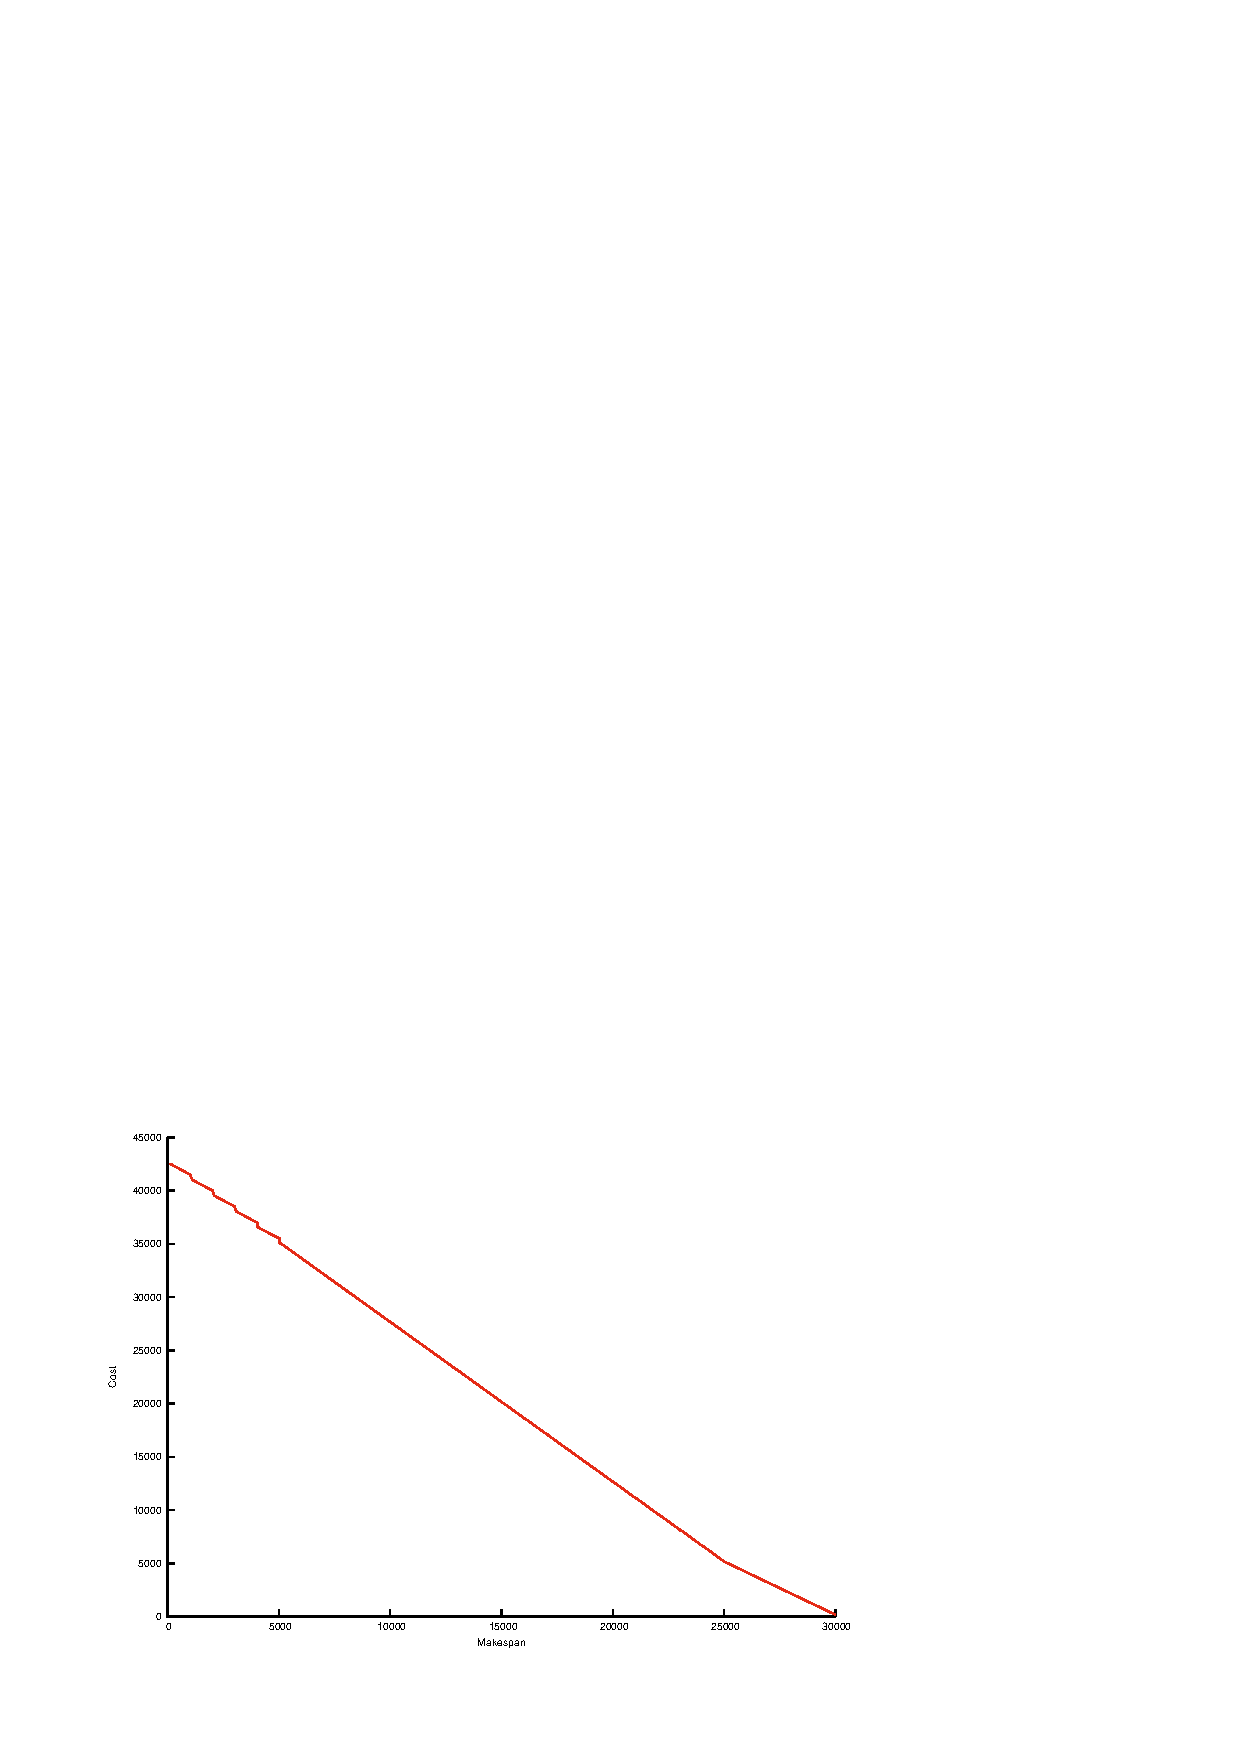
\includegraphics[width=0.30\textwidth]{9}
      \includegraphics[width=0.30\textwidth]{9_zoom}
 \caption{\label{instance6} Instance 3: quite linear, a zoom shows a non uniform repartition of points. Clusters of points seems to be regular all over the front.}
\end{figure}
\begin{figure}[h!]
  \centering
      \includegraphics[width=0.30\textwidth]{6}
      \includegraphics[width=0.30\textwidth]{6_zoom}
 \caption{\label{instance3} Instance 4: a concave trend. The lower part is quite regular while the upper part shows a non uniform and non regular distribution of points. We also notice a smaller concave part in the middle of the front that breaks the symetry of the general trend.}
\end{figure}
\begin{figure}[h!]
  \centering
      \includegraphics[width=0.30\textwidth]{8}
      \includegraphics[width=0.30\textwidth]{8_zoom}
 \caption{\label{instance4} Instance 5: it looks like Instance 3. However, the distribution of points is regular and uniform.}
\end{figure}
\begin{figure}[h!]
  \centering
      \includegraphics[width=0.30\textwidth]{7}
 \caption{\label{instance5} Instance 6: quite few points compared to the complexity of the instance. This is due to the effect of the ratio $\frac p t$.}
\end{figure}

\begin {table}[H]
\centering
\caption{\label{param} Instance parameters}
\begin{tabular}{|c|c|c|c|c|c|c|}
  \hline
  Instance & Cities & Pass. & Planes & \multicolumn{2}{|c|}{Generating functions} & Pareto Size \\
  \hline
  Instance 1 & 20 & 6 & 2 & \multirow{3}{*}{
\begin{tabular}{c}
$\frac{5}{2}i +$ \\
$ \frac{(i ~\text{mod}~ 2)}{10}$
\end{tabular}
} & \multirow{3}{*}{
\begin{tabular}{c}
$\frac{5}{2}i +$ \\
$ \frac{(i ~\text{mod}~ 2)}{10}$
\end{tabular}
} & 409 \\
  Instance 2 & 3 & 21 & 2 &  & & 61 \\
  Instance 3 & 10 & 10 & 3 & & & 383 \\ \hline
  Instance 4 & 200 & 3 & 2 & $log(i)$ & $\sqrt i$ & 538 \\
  Instance 5 & 200 & 3 & 2 & $log(i)$ & $log(i)$ & 399 \\
  Instance 6 & 8 & 26 & 25 & $\sqrt i$ & $i$ & 15 \\
  \hline
\end{tabular}
\end{table}

% \begin {table}[H]
% \centering
% \caption{\label{genfunc} Generating functions}
% \begin{tabular}{|l|c|c|}
%   \hline
%   Instance & $f$ & $g$ \\
%   \hline
%   Instance 1,2,3 & $f(i) = \frac{5}{2}i + \frac{(i ~\text{mod}~ 2)}{10}$ & $g(i) = \frac{5}{2}i + \frac{(i ~\text{mod}~ 2)}{10}$ \\
%   Instance 4 & $f(i) = log(i)$ & $g(i) = \sqrt i$ \\
%   Instance 5 & $f(i) = log(i)$ & $g(i) = log(i)$ \\
%   Instance 6 & $f(i) = \sqrt i$ & $g(i) = i$ \\
%   
%   \hline
% \end{tabular}
% \end{table}

\section{Experimentations using \DAEYAHSP}
\label{sec:exp}
\subsection{Divide-and-Evolve}
\label{sec:dae}

Based on the Divide-and-Conquer paradigm, this generic hybrid evolutionary approach has been originally introduced in~\cite{Schoenauer2006}.   
It splits the problem into a sequence of problems that are hopefully easier to solve by local search based heuristic. 
The initial sequence corresponds to an ordered subgoals to reach which are passed to the embedded heuristic; if all those subgoals are attained, the concatenation of all corresponding sub-plans is a solution of the initial problem.

The main idea to solve a planning task ${\cal P}_D(I,G)$ is to find a sequence of states $S_1, \ldots, S_n$, and to use some embedded planner to solve the series of planning problems ${\cal P}_D(S_{k},S_{k+1})$, for $k \in [0,n]$ 
(with the convention that $S_0 = I$ and $S_{n+1} = G$).
The generation and optimization of the sequence of states $(S_i)_{i \in [1,n]}$  is driven by an evolutionary algorithm, where the   sequence of subproblems ${\cal P}_D(S_{k},S_{k+1})$ are solved by an external 'embedded'
planner. The concatenation of the corresponding plans  (possibly with some compression step) is a solution of the initial problem.\\

Our algorithms have been hybridized with an external ’embedded’ planner to solve the sequence of problems ${\cal P}_D(S_{k},S_{k+1})$,  for $k \in [0,n]$. 
Any existing planner can be used as embedded planner, but since guaranty of optimality at all calls is not mandatory in order for \DAE\ to obtain good quality results~\cite{Bibai2010}, a sub-optimal, but fast planner is used: \YAHSP~\cite{Vidal2004} is a lookahead 
strategy planning system for sub-optimal planning which uses the  actions in the relaxed plan to compute reachable states in order to speed up the search process.

\subsection{Experimental Conditions}

Previous work \cite{khouadjia:hal-00750560} showed that using IBEA$_{H^-}$ as the evolutionary algorithm for DAE$_{\text{YASHP}}$ outperforms most of other evolutionary algorithms such as NSGA-II, SPEA2 or IBEA$_{\epsilon^+}$. This is the reason why all experiments have been conducted with IBEA$_{H^-}$. DAE$_{\text{YASHP}}$ internal parameters have been tuned thanks to \PARAMILS\ using an {\bf Hypervolume Difference Indicator} metric $H^-$. For further details about the tuning purposes and procedure, refer to \cite{khouadjia:hal-00820617}. For each instances, 20 runs based on 5400 seconds (except instance 6 based on 1800 seconds) have been performed. All performance assessment and metric have been achieved using the performance assessement tool suite provided by PISA\footnote{http://www.tik.ee.ethz.ch/pisa/}. %\cite{Bleuler2003}.

\subsection{\DAEYAHSP\ on Large Instances}

The attainment surface on Instance 1 shows that we can easily guess the exact Pareto shape. Few points are found and only with a probability lower than 20\% (except one extreme point). However, it seems that the attainment surface are uniformly distributed over the front. Surfaces on Instance 2 and 3 are far from the exact front and only 2 points are found for Instance 4 over 538. On the contrary, even if runs are shorter, results on Instance 6 are better since most of the points are found, except on the most concave part. Even is there is few points, the front remains well distinguishable with a good probability.

We can notice that, even if $n$ is higher for the Instance 6 than for the Instance 2, more planes results in a easier front to reach. This is quite surprising since the search space \DAEYAHSP\ for is growing with $p$. A reason could be the maximum number of states in a decomposition that has been fixed at 20 and could be too low to obtain easy-to-solve sub-problems, resulting on poor results on the Instance 2 and 3.

\begin{figure}[h!]
  \centering
      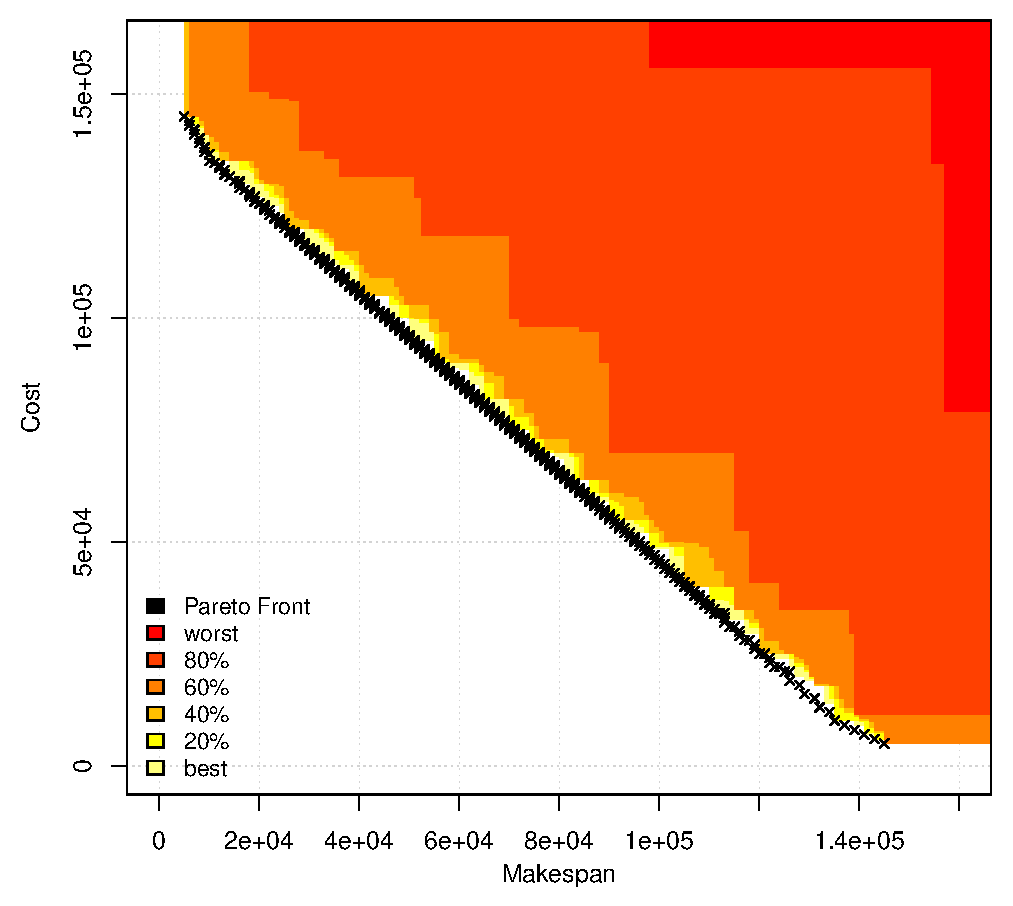
\includegraphics[width=0.30\textwidth]{large_1_att_area}
      \includegraphics[width=0.35\textwidth]{large_1_hyp}
 \caption{\label{instance5} Attainment surface and Hypervolume for Instance 1}
\end{figure}

\begin{figure}[h!]
  \centering
      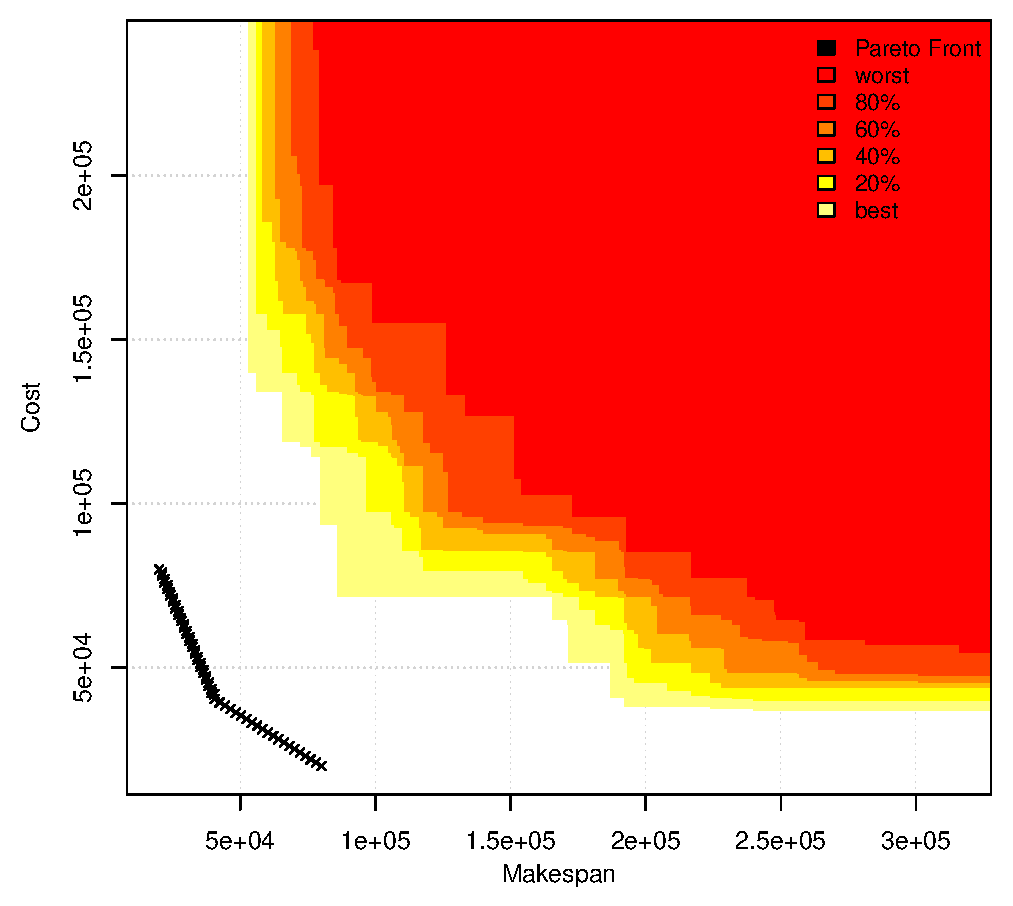
\includegraphics[width=0.30\textwidth]{large_4_att_area}
      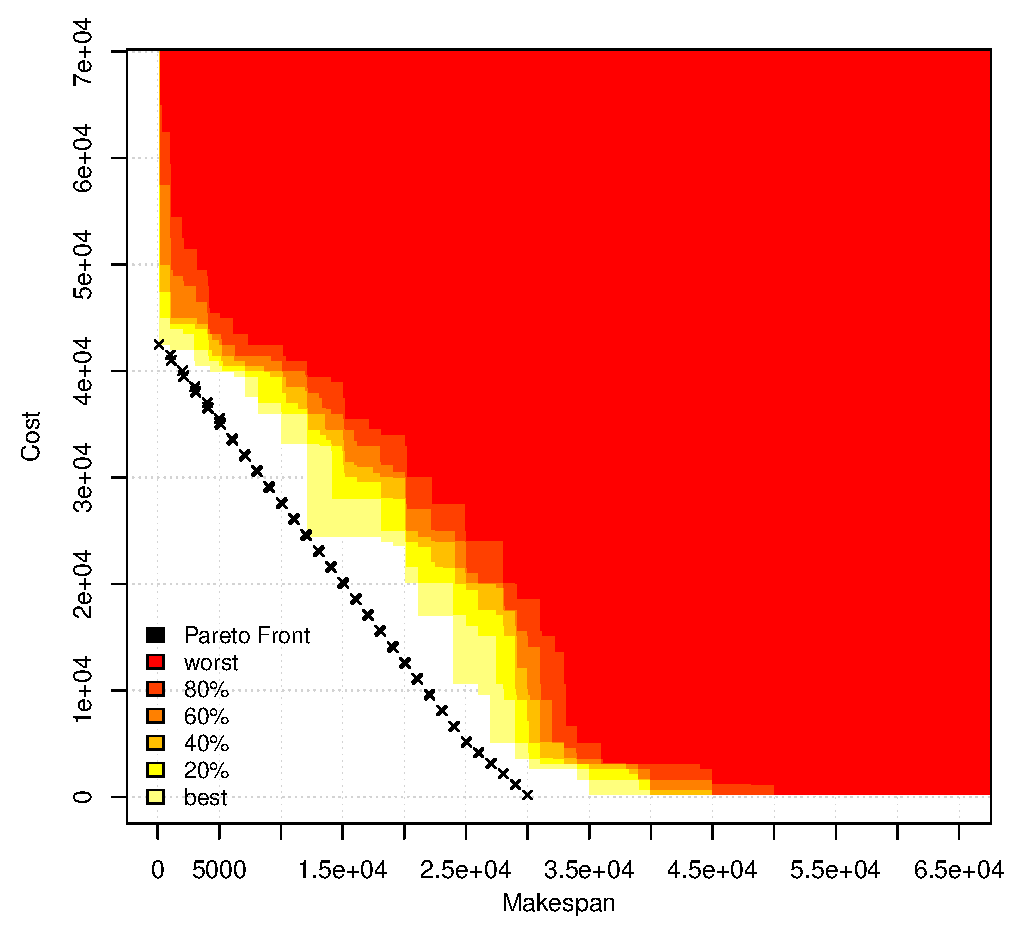
\includegraphics[width=0.30\textwidth]{large_9_att_area}
      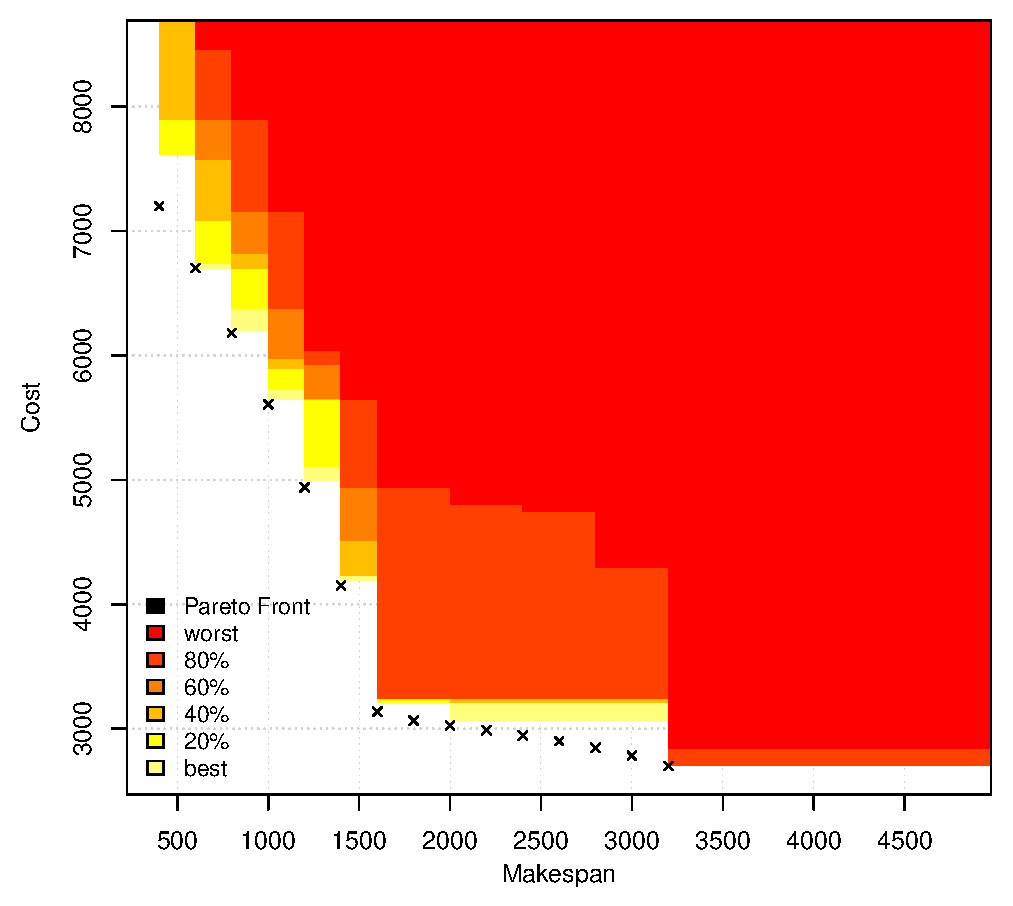
\includegraphics[width=0.30\textwidth]{large_7_att_area}
 \caption{\label{instance5} Attainment surface for Instance 2, 3 and 6.}
\end{figure}

\subsection{Comparing Aggregation against Pareto Approaches}

We present here a comparison between an aggregation of objectives and a Pareto approach on a concave instance based on same parameters as Instance 4, but using only 30 cities instead of 200. Thus, the Pareto Front is made of 66 points. Both approaches are performed by \DAE\ and previous work concerning such a comparison can be found in \cite{khouadjia:hal-00820617,khouadjia:hal-00820634}.
The attainment surfaces (see Figure \ref{medium_eaf}) show that in the case of Pareto approach, the exact Pareto Front is already distinguisable after 900 secondes, even considering only the worst run. On the contrary, even considering only the best run, in the case of aggregation, the Pareto Front shape is hard to guess. Naturally, there is a few points in fronts found by the aggregation and the only points belonging to the exact front remains outside of concave part while IBEA$_{H^-}$ found large sets on the whole exact front as shown by cumulated fronts on Figure \ref{medium_cum}.

\begin{figure}[h!]
  \centering
      \includegraphics[width=0.30\textwidth]{medium_att_area_EAFALL_900}
      \includegraphics[width=0.30\textwidth]{medium_att_area_EAFALL}
      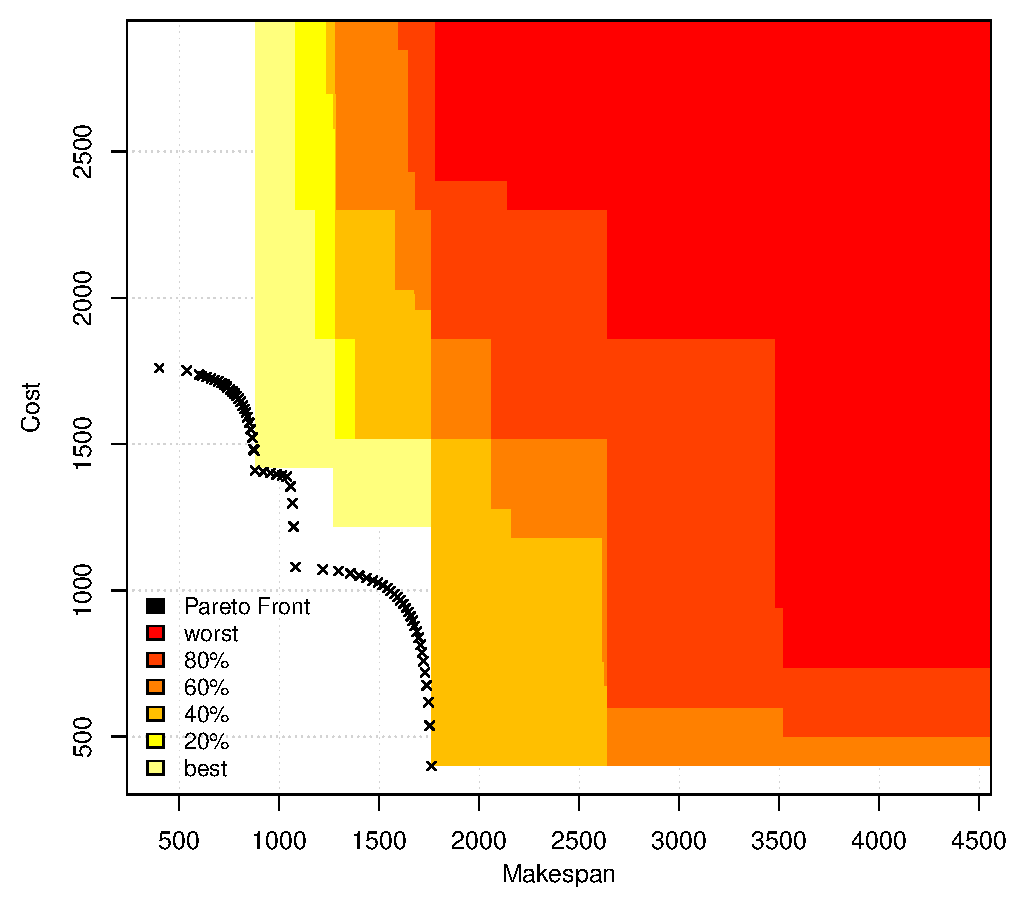
\includegraphics[width=0.30\textwidth]{medium_aggreg_att_area}
 \caption{\label{medium_eaf} Attainment surface for Pareto approach after 900 and 5400 seconds (left, center) and for aggregation after 5400 seconds (right).}
\end{figure}

\begin{figure}[h!]
  \centering
      \includegraphics[width=0.35\textwidth]{medium_cumulated}
      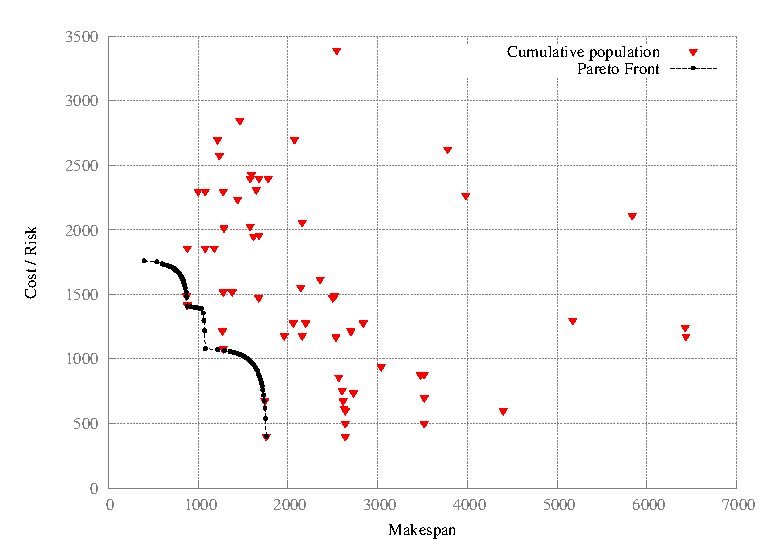
\includegraphics[width=0.35\textwidth]{medium_aggreg_cumulated}
 \caption{\label{medium_cum} Cumulated pareto fronts for Pareto (left) and aggregation (right).}
\end{figure}

The EAF difference plot indicates attainment surfaces more likely to be reached by an algorithm compare to another. On this concave instance, the parts in favor of the Pareto approach are always closer to the exact front that for the aggregation one. Thus, it is clear that the Pareto approach strongly outperforms the aggregation one and point out the difficulty of aggregation methods to reach concave parts of Pareto Front.

\begin{figure}[h!]
  \centering
      
      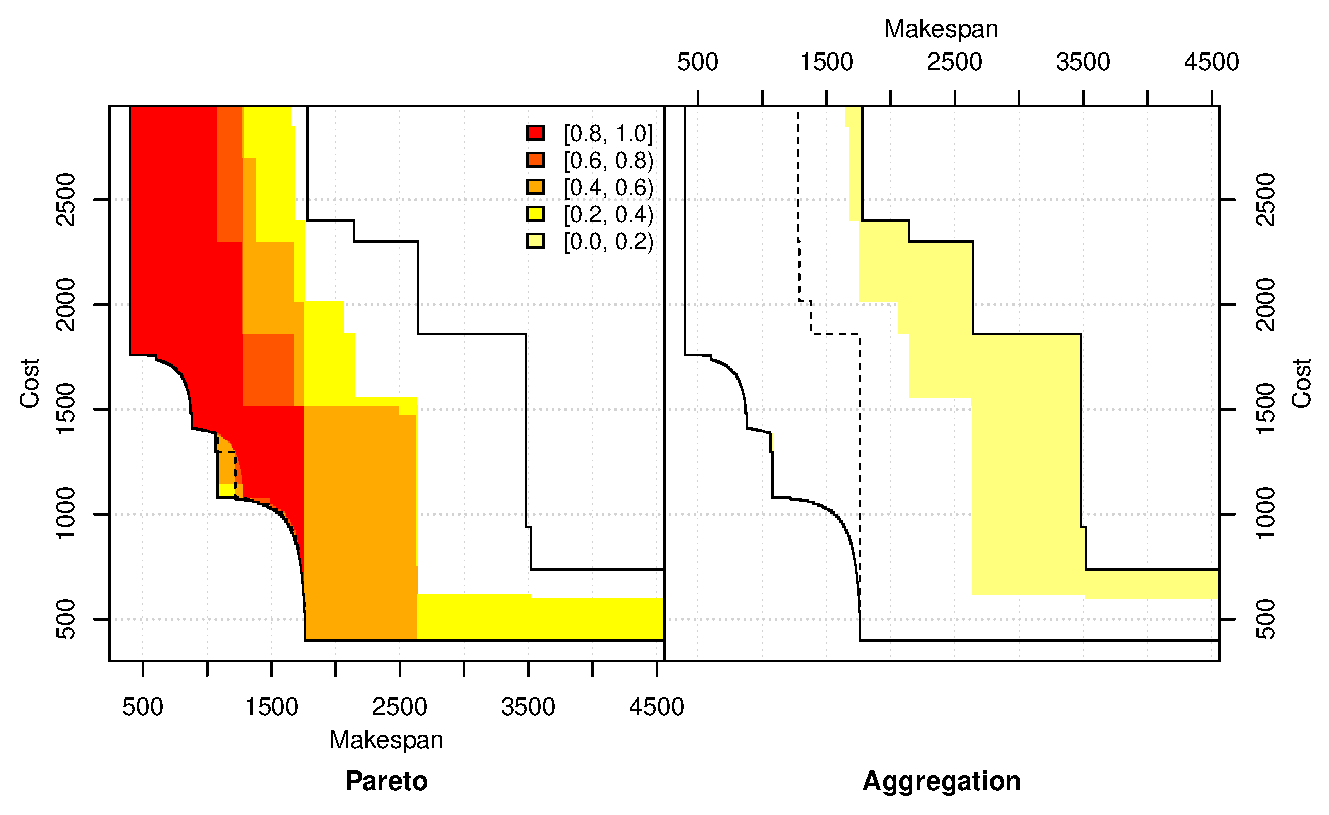
\includegraphics[width=0.6\textwidth]{medium_eaf_diff}
 \caption{\label{medium_diff} EAF difference between Pareto and Aggregation approches.}
\end{figure}

\section{Conclusion and Perspectives}
\label{sec:conclusion}

%
% ---- Bibliography ----
%
\bibliographystyle{splncs}
\bibliography{ppsnb}
%
\end{document}
